\documentclass{article}

\usepackage{parskip}
\usepackage{graphicx}
\usepackage[position=bottom]{subfig}

\begin{document}
	\section{Wavelets}
	13th July
	Collection and summary of various notes.
	\subsection{Introduction}
		
		\textbf{Transforms} - these are applied to singals to obtain further insights about the signals not available from the raw signal itself. A \textbf{time-domain} signal is basically a signal that can be plotted on an xy chart such that time is on the x-axis and amplitude is on the y-axis.
		
		\textbf{Time-amplitude} representation is not the best.
		The \textbf{frequency spectrum} of a signal refers to the frequency components (or \textbf{spectral} components) of a signal. It shows what frequencies exist in the signal. Frequencies can be high or low, and are measured in hertz (Hz).
		
		\textbf{Fourier transforms} (FT) lets us find the frequency content/spectrum of signal. FT gives the \textbf{frequency-amplitude} representation of a signal. 
		It should be noted that both FT and wavelet transforms (WT) are \textbf{reversible transforms}. In other words, we can go back and forth from the raw and transformed output. So, FT gives frequency information existing in a signal, but it does not tell us when in time do these signals exist. 
		
		\textbf{Stationary signals} are signals whose frequency content do not change in time. There is therefore no need to know at what point in time do which frequencies exists, because these frequencies exist at \textit{all} times.
		
		FT gives the spectral contents of the signal but does not give any information relating to where in time do the contents appear. Therefore, FT can be used in non-stationary singals only if we care about what spectral components exist and \textit{not} when in time do they occur. Therefore, when time localization is required, a different transform giving the time-frequency representation is needed.
		\subsection{Wavelets}
		Wavelet transforms (WT) provides a \textbf{time-frequency} representation, and were developed as an alternative to overcome the resolution issues inherent in the Short time Fourier Transform. 
		
		\subsubsection{Short Time Fourier Transform: A Digression}
		
		In order to develop the idea of the WT, we first introduce the \textbf{Short time Fourier Transform (STFT)} and the \textbf{decomposition} operation.
		
		The idea of decomposition is as follows: Suppose we have a time-domain signal with has frequencies up to 1000 Hz. By using high-pass and low-pass filters, we can filter out the high and low frequency parts of the signal respectively. We split this signal into 2 constituent signals by passing the signal into both filters, which then results in 2 different versions of the same signal: A signal in the 0-500 Hz (lowpass portion) and another in the 500-1000 Hz (highpass portion). We take the lowpass portion and put it into the high- and lowpass filters again, this time obtaining 2 parts 0-250 Hz in the lowpass portion and 250-500 Hz in the highpass portion. The process of repeatedly passing the signal into the filters which \textit{splits} the signal into smaller parts is called \textbf{decomposition}. 
		
		Therefore by the decomposition operation, we can take a signal and split it up into different pre-defined frequency bands. So by repeatedly passing a time-domain signal into various high-pass and low-pass filters, every time, some portion of the signal corresponding to a certain band is removed each time. 
		
		By combining each of these bands, we are able to get a 3-D represention in terms of time, frequency and amplitude. However, it is important to note here that we are no longer working with specific frequencies but instead frequency bands: while we can't say exactly which frequencies exist at which exact time instance, we can however say which frequency bands exist at which time intervals. 
		
		This idea is very closely linked to the \textbf{uncertainty principle} by Heisenberg states that the momentum and position of a moving particle cannot be known simultaneously. In the context of our above experiment, we cannot know for sure what spectral component exist at any time \textit{instant}; instead, we can know what spectral component exist at any given \textit{interval} of time.
		
		\subsubsection{Frequency Resolution}
%		So looking at the limitations \textbf{Short Time Fourier Transform} (STFT), we switch to using WT due to resolution issues. STFT has a fixed resolution, while WT is variable. 
		
		High frequencies are better resolved or detected in \textit{time} than low frequencies. This means that a high frequency component can be picked out in time with lower errors than a low frequency component.
		
		On the other hand, low frequencies are resolved in \textit{frequency} with lower errors than high frequencies.
		
		\begin{figure}[!t]
			\centering
			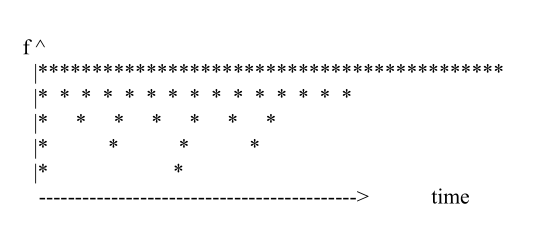
\includegraphics{img/hi_freq_resol_1}
			\caption{High frequencies are better resolved in time}
			\label{fig:hi_freq_resol_1}
		\end{figure}
		
		To motivate the first point, consider a time-frequency plot and assume stationary signals. Fig. \ref{fig:hi_freq_resol_1} shows a continuous WT. From it, note how the spacing between asterisks increase with frequency: we can see that the high frequency signal is formed by a solid line of asterisks, which allows it to clearly stand apart from the rest of the lower frequency signals. The higher frequency signal can be thought of as \textit{having more samples per unit time.} For the lower frequencies, we see that the signals are 'clustered' together and it is hard to pick any one out from the rest. For the discrete WT case, the idea is essentially the same.
		
		\begin{figure}[t!]
			\centering
			\subfloat[Sinusoidal example with 2 frequencies]{
				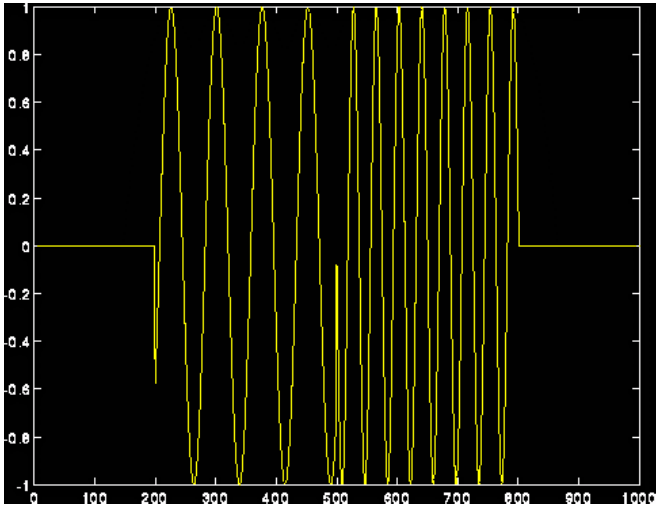
\includegraphics[width=0.4\textwidth] {img/lo_freq_resol_1}
				\label{fig:lo_freq_resol_1} } 
			\hspace*{2.0em}
			\subfloat[3-D representation in terms of scale, amplitude and translation]{
				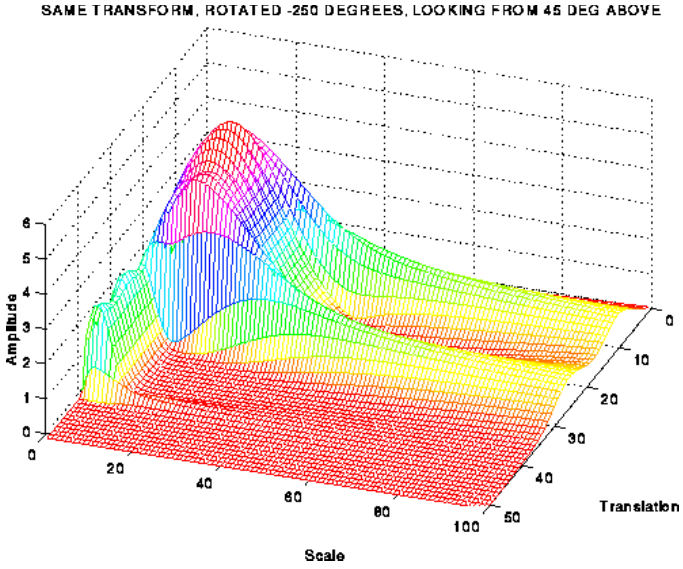
\includegraphics[width=0.4\textwidth] {img/lo_freq_resol_2}
				\label{fig:lo_freq_resol_2} } \\
			\caption{Resolution of Low Frequencies}
			\label{fig:lo_freq_resol}
		\end{figure}
	
		For the second point, we make use of a sinosoidal signal with 2 frequencies (See how the waves are more compressed on the right half) as shown in Fig.  \ref{fig:lo_freq_resol_1}. One key thing to note in Fig. \ref{fig:lo_freq_resol_2} is that \textbf{scale} is the \textit{inverse} of frequency. The small bumps may lead us to think that high frequency (small scales) are easy to pick out. However this brings us to  a very important point: Good scale resolution means poor frequency resolution and vice versa. 
		
	\subsection{Fourier Transform}
	
	This section touches on the FT briefly. 
	
	Recall that FT is not suitable for non-stationary signals. Since the FT gives only a amplitude- frequency, it does not capture the fact that the properties of the signal may be changing in time.

		
		
		
		
		
	
	
	
\end{document}